\chapter{Introduction}\label{chap:intro}

Since the industrial revolution, our demand for energy has only increased.
In the early part of the last century, the only option for extracting usable energy has been by burning fossil fuels, such as coal and natural gas. Unfortunately, the by-product of burning these fossil fuels, carbon dioxide, is a greenhouse gas that traps heat. The ecological effects of this increased store of energy in our atmosphere has already begun. 
Fortunately, we now have better options than burning fossil fuels, although they are not without their problems.

\section{Alternative Energy: The Past and Present}
\subsection{Hydroelectric Power}
Hydropower is one of the oldest form of energy extraction, having been used in ancient times to grind grains and do other tasks. In modern times, the first industrial plant to use hydropower to produce electricity, Schoellkopf Power Station No. 1, was completed in 1881 near Niagara Falls\cite{schoellkopf}. Hydroelectric power generation is an attractive source of energy as it does not produce carbon dioxide although it has several other issues which limits its use. The first issue is the limited locations where hydroelectric power can be effectively utilized. Due to transmission losses, power plants should be placed near high population centers; however, this is not always possible as the locations of possible plants are determined by the flow of a river and the topology of the land. The second issue with hydroelectric power is its ecological and archaeological impact. Hydropower extracts energy from a gravitational potential difference. In the absence of a natural potential difference, such as a waterfall, an artificial one in the form of a dam must be built. The consequent flooding of the area preceding the dam causes the aforementioned ecological and archaeological problems. These issues are not theoretical. Take for example the creation of Lake Powell in the American west. Lake Powell was created by the flooding of Glen Canyon by the construction of Glen Canyon Dam. Before the flooding, Glen Canyon contained over 80 side canyons, clear streams, abundant wildlife, arches, natural bridges, and numerous Native American archaeological sites. All that history and natural splendor was lost under the water.

\subsection{Wind Power}
Wind power is nearly as old---if not older---than hydropower, having been used by sailors since time immemorial to push their ships across the water. The first electric generator to use wind power was built in Scotland in 1887 by Professor James Blyth of Anderson's College\cite{price2005james}. Although not as prolific as hydroelectric power is, wind power is still an attractive energy source as it has no by-products and has minimal environmental impact if you discount the effects on migratory patterns and on the views of rich people\cite{cape_cod_wind}. However, like hydroelectric power, wind power is location limited as there are limited places where there is persistent wind. Also, unlike hydroelectric power, the rate of power generation can be highly variable---a consequence of the variability of wind strength. The volatility of wind power causes strain on the electrical grid. The technological advances over the last few decades has blunted much of this volatility. However, even with recent improvements that has made wind more viable, it doesn't change the fact that if there is no wind, there is no power. A form of energy that does not depend on the weather---which is itself becoming more volatile due to global warming---is required.

\subsection{Nuclear Fission Power}
After the bombing of Hiroshima and Nagasaki and the subsequent end of World War II, the use of nuclear fission for electricity generation was promoted as a peaceful use for the technology that had only known bloodshed. The first nuclear reactor, Chicago Pile-1, was developed during the Manhattan project in 1942. Chicago Pile-1 generated no electricity and it wouldn't be until 1951 that the EBR-I experimental reactor produced electricity\cite{doe_nuclearhistory}. It would take another three years and a different country to build a reactor that connected to the electrical grid---USSR's Obninsk Nuclear Power Plant. In the following years, many nuclear fission plants were built. However, the number of plants being built drastically decreased in latter part of the 20th century. This was due to economic, regulatory, ecological, and public perception issues.

Nuclear fission power has few flaws. Unfortunately, those flaws are of the fatal variety. Unlike wind power, nuclear fission power can provide a steady flow of electricity for an extended period of time. Additionally, unlike hydroelectric power, there are few technical limitations on where a plant can be built. The problem that doomed nuclear fission power was the uranium fuel it used and the subsequent long lasting radioactive waste it produced. There is a limited amount of fissionable material available on Earth. The mining and subsequent refining of the fuel greatly increases the cost. Additionally, the ability to use the fuel and waste for a bomb, the health issues caused by radiation exposure, and the possibility of a uncontrolled nuclear meltdown requires strong regulatory oversight. This oversight, while necessary, is a strong economic disincentive. Furthermore, while there are few \textit{technical} limitations on where a plant can be built, there are numerous societal limitations---no one seems to want a nuclear fission reactor in their neighborhood. Combined with the difficulties in storing the waste, both perceptual and practical, nuclear fission power has shown itself to not be economically viable.

\subsection{Solar Power}
Solar power is perceived to be a relatively recent energy source. This impression probably stems from the recent proliferation of the technology due to increases in efficiency---and government subsidies---as well as decreases in manufacturing costs. Contrary to public perception, solar power has a rich history dating back over a century. The photovoltaic effect was first observed by Alexandre Edmond Becquerel in 1839 when he, at the age of 19, placed silver chloride into an acidic solution connected to platinum electrodes. When illuminated, a voltage and current were generated; creating the first photovoltaic cell.\footnote{The related photo\textit{electric} effect was first observed by Heinrich Hertz in 1887} The first use of what we would call solar panels was not until 44 years later when in 1883 Charles Fritts created an array of selenium based solar cells and placed them atop a New York City rooftop\cite{historyofenergy}. The efficiency of these first solar panels were about 1\% and extremely expensive. In contrast, today's best silicon-based solar panels are over 40\% efficient. Despite the experimental successes, we did not understand the physics behind the photovoltaic effect---and the related photoelectric effect---until Albert Einstein explained the effect using quantum theory in the first of his ``Annus Mirabilis'' papers in 1905. It was this work that earned Einstein the Nobel Prize in 1921.

\begin{figure}[ht]
    \centering
    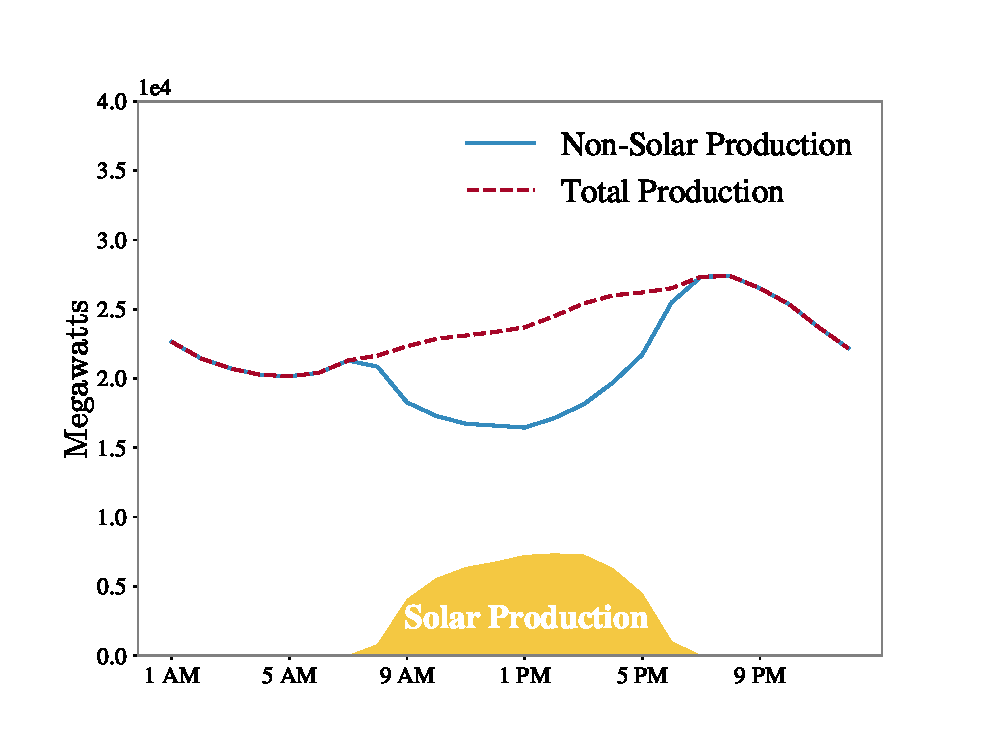
\includegraphics[width=13cm]{duck_curve.eps}
    \caption{Energy production in California on October 22, 2016.\cite{caiso} Total production is lowest in the early hours of the morning and peaks in the evening. Solar production peaks in the middle of the day.}
    \label{fig:duck_curve}
\end{figure}
Of all the previously discussed energy extraction technologies, solar has the fewest issues, after all, its hard to complain about free energy raining from the sky---in fact, most of the work since 1905 has been in designing the best bucket to capture it in. However, solar does have its foibles. Apart from solar's obvious and most nefarious enemy, the cloud, much of solar's issues lie in its interface with the existing electrical grid and its relatively low energy density. Since solar does not produce energy during the night, conventional fossil fuel plants need to pick up the slack. In the presence of solar power, these base load providers see a large dip in demand during the day (Fig. \ref{fig:duck_curve}), the time when solar is providing a significant portion of the electricity. Peak electricity usage ramps up in the late afternoon and peaks in the evening hours, precisely when solar production is decreasing. This means the base load providers have to quickly ramp up from a very low production level to a very high production level. This is not always possible and this problem only gets worse with more solar panels connected to the grid. Additionally, most base load providers are only economical if they produce a certain amount of electricity 24/7. If solar provides more electricity than the grid can handle, service managers would have to shutoff some of the panels to avoid damaging the grid; wasting electricity. This problem is exacerbated by the highly distributed nature of solar---solar requires a large collection area and, since there are few large open fields near major population centers, many smaller solar installations are installed. While most of these issues could be resolved with a better designed electrical grid, the fact remains that solar doesn't work at night and fossil fuel burning base load providers have to be utilized. Solar only solves the problem during the day. To solve the problem during the night, we have to look towards a new technology. 

\section{Alternative Energy: Possible Future}
A good alternative energy power plant should not subject to the whims of the weather, be energy dense both in terms of the fuel and in terms of the power plant itself, location independent, and produce no long lasting harmful by-products, e.g. carbon dioxide and nuclear waste. These criteria precludes all of the previously discussed energy sources. Fortunately, there is an energy source in development that meets most of the criteria: nuclear fusion. Unlike nuclear fission, fusion fuel does not produce any long lasting radioactive waste nor does it produce carbon dioxide. There is also no possibility of a meltdown and it uses less fuel. It has all the benefits of fission without many of its problems.

\subsection{Nuclear Fusion}
In nuclear fission, larger nuclei are split, creating smaller nuclei. Fusion is the opposite process in which we take lighter nuclei and fuse them together to create heavier nuclei. In either process, energy is released. To understand where this energy comes from we must consider the nature of the nucleus, particularly how the protons and neutrons are held together. There are two opposing forces at play in a nucleus: the strong force, which keeps the nucleus together, and electromagnetic force, which wants to tear the nucleus apart. This dance of forces means that every nuclei has an internal energy level---a consequence of quantum mechanics.
We can represent this energy level using the binding energy of the nucleus (Fig. \ref{fig:binding_energy}). The binding energy is the work required to disassemble the nucleus. The \textit{larger} the binding energy, the \textit{lower} the nucleus's energy level. We can change the energy level of a nucleus by adding or removing nucleons---protons or neutrons. If the change results in an lower energy state, then the excess energy is released in the form of kinetic energy. The amount of energy released is given by the difference in the binding energy of the starting and ending nuclei. According to Figure \ref{fig:binding_energy}, there is only two ways to release energy from a nucleus: start with a heavy element and reduce its mass (fission) or start with a light element and increase its mass (fusion).
\begin{figure}[h!]
    \centering
    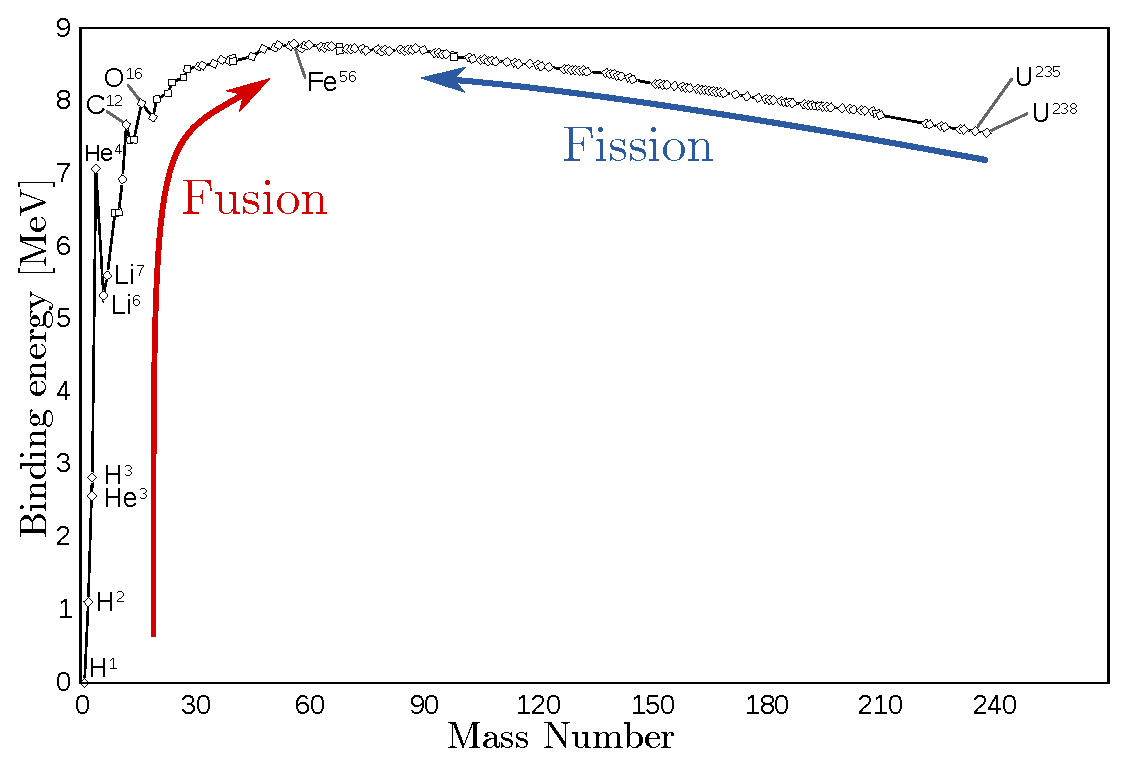
\includegraphics[width=13cm]{annotated_binding_energy.eps}
    \caption{Binding energy of nuclei. A change in the binding energy releases kinetic energy.}
    \label{fig:binding_energy}
\end{figure}

As can be seen in Figure \ref{fig:binding_energy}, fusion releases much more energy than fission per nucleon added. So what lighter elements should we fuse? Before we answer that, there are a few things we must consider: the energy needed to fuse, which we want to minimize; the output energy, which we want to maximize; and the cross section or probability of the interaction, which we also want to maximize. With these three criteria in mind, there are three particularly attractive candidate fuels: Deuterium--Tritium (D-T), Deuterium--Deuterium(D-D), and Deuterium--He$^3$(D-He$^3$). Table \ref{tab:fuel} shows the possible fuels and their properties.
\begin{table}[ht]
    \centering
    \caption{Possible fusion fuels. Due to its relatively large cross section at expected burning temperature and energy gain D-T fuel is the most achievable option. However, the Coulomb scattering cross section is orders of magnitude larger than the fusion cross sections. Because of this, the fuel is much more likely to just bounce off each other than fuse.}
    \label{tab:fuel}
    \begin{tabular}{cccc}
        \textbf{Fuel} & \textbf{Exhaust} & \textbf{Energy Gain} & \textbf{Cross Section @ 15 keV} \\ \hline \hline 
        D + T & $\alpha$ + n & 17.6 MeV & $1.48 \times 10^{-1}$ b \\[5pt]
        D + D & \begin{tabular}[c]{@{}c@{}}T + p (50\%)\\ He$^3$ + n (50\%)\end{tabular} & 3.65 MeV & $1.18 \times 10^{-3}$ b \\[10pt]
        D + He$^3$ & $\alpha$ + p & 18.35 MeV & $7.94 \times 10^{-6}$ b \\[5pt] \hline
    \end{tabular}
\end{table}
Figure \ref{fig:scattering} shows the cross sections of the different fusion fuels as a function of energy. The D-T fusion cross section is consistently larger than the other fuels and this, coupled with the large energy gain, lends itself to be the fusion fuel of choice.

However, if fusion was just a matter of colliding the fuel together at high energy, we would of achieved fusion decades ago; after all, CERN routinely collides particles together at TeV energies---more than enough for fusion to occur. The issue is that the Coulomb scattering cross section is orders of magnitude larger than the fusion cross sections (Fig \ref{fig:scattering}). This means that it's much more likely that the fuel will bounce off each other than fuse. Its rather like playing pool without the bumpers. The probability of getting a ball in a pocket is rather small. It's much more likely the ball will fall off the table and go out of play. However, if we put the bumpers back on, the balls become confined and we have more opportunities for getting a ball in a pocket. Likewise, if we contain the fuel, it will have more chances to fuse.
\begin{figure}[ht]
    \centering
    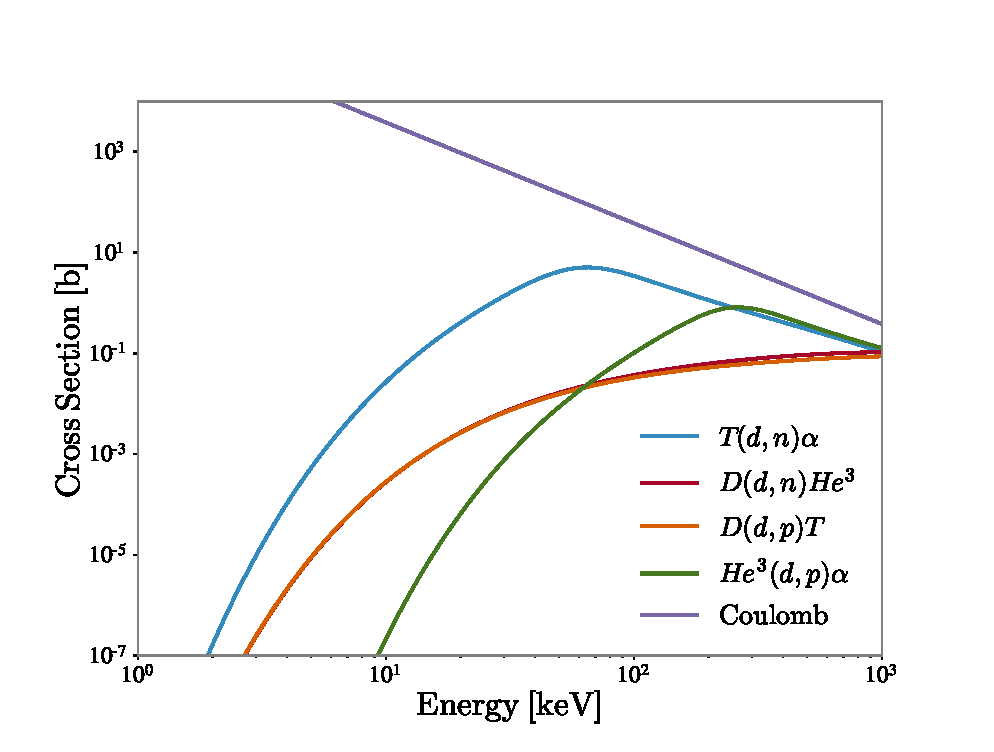
\includegraphics[width=13cm]{cross_sections.eps}
    \caption{Fusion and Coulomb scattering cross sections.}
    \label{fig:scattering}
\end{figure}
When contained and heated, the fuel becomes a plasma, a hot gas composed entirely of ions and electrons. Unlike other materials whose dynamics of motion are determined by forces between neighboring regions, the charge separation that exists in plasmas give rise to electromagnetic fields, which results in complex collective phenomena.

Designing a reactor that can effectively contain the plasma at the required temperatures is difficult and it is not yet clear that this can be done in a cost effective manner. Just having materials that can withstand a fusion environment is still an open area of research. Additionally, while the fuel itself does not produce any long lasting radioactive waste, it does produce high energy neutrons, which can irradiate reactor materials and compromise structural integrity. This leads to reactor components having a finite lifetime, after which the irradiated material needs to be stored, similar to fission. Fortunately, the amount of waste is considerably less than the amount produced by fission and has a shorter half-life. Fusion reactors also have more flexibility in regards to the materials used than fission reactors. This allows fusion reactors to use materials that are less susceptible to being irradiated. For instance, Vanadium is much less susceptible to being irradiated than stainless steel. However, research into the various Vanadium alloys for use in fusion reactors has been limited. 

The fusion fuel may also be a problem. While Deuterium is abundant, there is only a small amount of Tritium on earth. Tritium can be made by bombarding Lithium with high energy neutrons, but there is not yet an infrastructure in place for large scale production. It has been suggested that a Lithium breeder blanket can protect the outer materials from the neutron flux, provide a way of extracting energy, and produce the Tritium needed, but the feasibility of such a design has not yet been demonstrated.

\begin{figure}
    \centering
    \includegraphics[width=12cm]{figures/fusion_never.png}
    \caption{Graph of U.S government magnetic fusion research budget compared to 5 funding scenarios from the 1976 Energy Research and Development Administration development plan.\cite{1976_fusion}}
    \label{fig:fusion_never}
\end{figure}
The aforementioned issues are not insurmountable; however, progress towards solving them is heavily dependent on the availability of funding. Unfortunately, fusion research has been chronically underfunded for decades. Since its inception in 1955, the U.S. fusion program has, adjusted for inflation, spent total of 42.6 billion\footnote{This figure includes both the budget for the magnetic and inertial confinement programs} dollars. To put this into perspective, NASA's 2018 budget was 20.7 billion dollars--just under half of the total amount spent on the fusion program over its entire 63 year history. Some may argue that we have spent too much on fusion research, but the reality is that we have spent too little. Figure \ref{fig:fusion_never} shows a graph of the budget for the U.S. Magnetic Fusion Energy program compared against five funding scenarios\cite{1976_fusion}. At the current levels of funding, there is a very real possibility that fusion energy will never exist---a hard truth that many young fusion scientists need to accept.
However, just because something is difficult doesn't mean its not worth doing. The benefits of fusion far outweigh its costs.

\subsection{Tokamaks}
\begin{figure}[ht]
    \centering
    \includegraphics[width=13cm]{tokamak.eps}
    \caption{Toroidal magnetic configuration of a tokamak. The toroidal field is provided by a series of field coils and the poloidal field is primarily generated by an electric current with a set of poloidal coils to assist with shaping. This fields give rise to a helical magnetic field which is necessary to maintain pressure balance. Figure modified from original\cite{geiger2013thesis}.}
    \label{fig:tokamak}
\end{figure}
In the 60+ years of fusion research, there have many different confinement schemes that have been tried. The most promising is the Tokamak.

Invented in the 1950's by Soviet physicists, the tokamak uses magnetic fields in a toroidal configuration to confine the plasma (Fig. \ref{fig:tokamak}). The principal toroidal magnetic field is provided by a series of field coils. In order to balance the plasma pressure, a current is run through the plasma to generate a poloidal field---additional poloidal field coils are also used for plasma shaping. The combination of the toroidal and poloidal field give rise to a helical magnetic field.

After an initial false start of disseminating their results in 1965, by 1969 the Soviet physicists had demonstrated that the tokamak outperformed all previous confinement schemes. A flood of small tokamaks were built in the following few decades. However, research showed that larger devices better contained the plasma and, as a result, many of the small tokamaks were decommissioned in favor of larger tokamaks. In the following sections, we will briefly discuss three of these larger tokamaks: DIII-D, ASDEX Upgrade, and NSTX-U.

\subsubsection{DIII-D}
\begin{figure}[ht]
    \centering
    \includegraphics[width=10cm]{DIII-D.jpg}
    \caption{DIII-D Tokamak}
    \label{fig:d3d}
\end{figure}
Located at General Atomics in San Diego, CA, the DIII-D tokamak(Fig. \ref{fig:d3d}) is currently the largest operating tokamak in the United States\cite{luxon2002design}.
Originating out of the Doublet III experiment, the DIII-D tokamak began operations in 1986. DIII-D is known for it advanced shaping capabilities, which allows it to achieve high plasma $\beta$\footnote{plasma $\beta$ is the ratio of the plasma pressure to the magnetic pressure} with a lower magnetic field. The plasma heated with 8 neutral beam injection (NBI) systems, which can provide up to 20 MW of heating. Additional heating is done via radio frequency (RF) injection in the forms of ion cyclotron resonance heating (ICRH) and electron cyclotron resonance heating (ECRH). DIII-D's operating parameters are given in Table \ref{tab:d3d}.
\begin{table}[h!]
    \centering
    \caption{DIII-D Operating Parameters\cite{luxon2002design}.}
    \label{tab:d3d}
    \begin{tabular}{ccccc}
        \textbf{Minor Radius} & \textbf{Major Radius} & \textbf{Magnetic Field} & \textbf{Heating} & \textbf{Current} \\ \hline \hline
        0.67 m & 1.67 m & 2.2 T & 23 MW & 2 MA \\ \hline
    \end{tabular}
\end{table}

\subsubsection{ASDEX Upgrade}
\begin{figure}[ht]
    \centering
    \includegraphics[width=12cm]{asdex.jpg}
    \caption{ASDEX Upgrade Tokamak\cite{geiger2013thesis}}
    \label{fig:augd}
\end{figure}
Beginning operation in 1991, ASDEX Upgrade(Fig. \ref{fig:augd}) is the successor to the successful \textbf{A}xially \textbf{S}ymmetric \textbf{D}ivertor \textbf{Ex}periment (ASDEX) which discovered the High-confinement operating mode (H-mode)\cite{wagner1982hmode}. It is currently the third largest fusion device in Europe, behind the Wendelstein 7-X stellarator\cite{wendelstein7x1993} and Joint European Torus (JET)\cite{jet1985}. It is comparable to the DIII-D tokamak. Up to 33 MW of heating power is provided by 4 NBI systems, ICRH, and ECRH. ASDEX Upgrade's operating parameters are given in Table \ref{tab:augd}. 
\begin{table}[]
    \centering
    \caption{ASDEX Upgrade Operating Parameters}
    \label{tab:augd}
    \begin{tabular}{ccccc}
        \textbf{Minor Radius} & \textbf{Major Radius} & \textbf{Magnetic Field} & \textbf{Heating} & \textbf{Current} \\ \hline \hline
        0.5 m & 1.65 m & 2.5 T & 33 MW & 1.4 MA \\ \hline
    \end{tabular}
\end{table}

\subsubsection{NSTX \& NSTX-U}
\begin{figure}[ht]
    \centering
    \includegraphics[width=10cm]{nstxu.jpg}
    \caption{NSTX-U Spherical Tokamak}
    \label{fig:nstx}
\end{figure}
Unlike the previous tokamaks, NSTX and its recent upgrade, NSTX-U, is a spherical tokamak. Spherical tokamaks have a much smaller aspect ratio: $R/a\sim1$ as opposed to $R/a\sim3-4$ in conventional tokamaks. A small aspect ratio allows spherical tokamaks to easily achieve high plasma $\beta$ with a low magnetic field. This could lead to smaller and more economical fusion reactors. NSTX began operation in 1999 and was upgraded in 2015. It is heated by NBI and ICRH. NSTX-U's operating parameters are given in Table \ref{tab:nstx}. 
\begin{table}[h!]
    \centering
    \caption{NSTX/NSTX-U Operating Parameters}
    \label{tab:nstx}
    \begin{tabular}{ccccc}
        \textbf{Minor Radius} & \textbf{Major Radius} & \textbf{Magnetic Field} & \textbf{Heating} & \textbf{Current} \\ \hline \hline
        0.68 m & 0.85 m & 0.3 T & 11 MW & 1.4 MA \\ \hline
    \end{tabular}
\end{table}

\subsection{The Lawson Criterion and Fast ion Confinement}
In order to maintain steady-state operation in the aforementioned tokamaks, the power going into the system must equal the power going out. There are several power sources in a tokamak. The power supplied by fusion, $P_{fusion}$, is broken up among its exhaust. For D-T fuel only the power from the alpha particles, $P_\alpha$, contributes to the power balance as the neutrons, having no charge, do not interact with the magnetic field and their power is deposited into the vessel wall or, in the case of a reactor, the blanket. Due to poor confinement and radiative emission, there is also lost power, $P_{lost}$. Additionally, if the power supplied by the fusion products is insufficient to keep the plasma going, external power, $P_{ex}$, must be supplied---usually in the form of NBI, ICRH, and ECRH. The power balance equation is then
\begin{equation}\label{eq:power_balance}
    \frac{dW}{dt} = P_\alpha + P_{ex} - P_{lost} = 0
\end{equation}
where $W$ is the energy density.

From this equation, we can extract a few useful concepts. In steady-state, the time it takes a plasma to dump all its energy, the energy confinement time, is given by
\begin{equation}\label{eq:tau_e}
    \tau_E = \frac{W}{P_{lost}}.
\end{equation}
From the power balance equation, we can also define the amplification factor, $Q$, which is the ratio of the fusion power and the external power: $Q = P_{fusion}/P_{ex}$. A $Q > 1$ is a minimum requirement in a fusion reactor, otherwise, more energy is put in than is generated. Most importantly, ignition---the point where the alpha heating is large enough to compensate for any losses---occurs when $P_\alpha > P_{lost}$. If the plasma ignites, it becomes self sustaining and external heating can be shut off---known as the burning plasma regime; a desirable quality in a reactor.
In order to ignite, the plasma has to be dense enough, hot enough, and confined for a long enough time. These conditions are codified in the Lawson Criterion---also derived from the energy balance equation---which can take the form of a triple product,
\begin{equation}\label{eq:lawson}
    nT\tau_E > \frac{12}{\langle \sigma v \rangle} \frac{T}{\mathcal{E}_\alpha} > 3\times10^{21} \; \rm{m^{-3}\, keV\, s}, \quad \rm{for\;D-T\;fusion}.
\end{equation}
There are many ways this criterion could be met, for example by having $n = 10^{20}\, \rm{m^{-3}}$, $T = 10\,\rm{keV}$, and $\tau_E = 3\,\rm{s}$.

To get into the burning plasma regime, one must first apply enough external heating to reach the ignition point. This is usually done through a combination of neutral beam injection and RF heating. This heating creates a small population of ions whose temperature is much greater than the background plasma. These fast ions start out at a high energy ($\sim 80$ keV) and through a series of collisions with the background plasma, thermalize. The process of thermalization transfers energy to the background plasma, increasing its temperature. The fast ions, while necessary to heat the plasma, bring with them a series of problems that need to be overcome in order to achieve fusion.

One of the main problems that fast ions bring is their ability to resonate with a class of instabilities called Alfv\'en eigenmodes\cite{heidbrink2008basic}. The fast ions that are resonant with the mode can either take energy away from the mode, making the plasma more stable and enhancing confinement, or, more commonly, they drive the instability, making the plasma more unstable and degrading confinement. In the presence of many Alfv\'en eigenmodes, fast ions are redistributed into regions where they are lost, either to the wall or through charge exchange with edge cold neutrals that exist in the outer layers of the tokamak. As a result, the fast ions transfer less energy to the thermal ions, which affects heating and also global confinement.\cite{heidbrink2014confinement,holcomb2015fast}

The fast-ion resonances occur in very particular regions in phase-space. In order to understand the wave-particle interactions, we need to know where the fast ions are relative to these resonances. This information is encoded in the fast-ion distribution function. Knowing the form of the fast-ion distribution function is the key to understanding not only wave-particle interactions but all of fast-ion physics.

The goal of this thesis is to infer the fast-ion distribution function from experimental measurements. The outline of the thesis is as follows. In Chapter \ref{chap:diagnostics}, we go over a few of the diagnostics that are sensitive to the fast ions. We discuss, in detail, how they encode information about the fast-ion distribution and how this information is translated via the diagnostics forward models into measurable quantities. In Chapter \ref{chap:fidasim}, we discuss the development of FIDASIM\cite{heidbrink2011code,geiger2013thesis,FIDASIM}, the practical implementation of the forward models discussed in Chapter \ref{chap:diagnostics}. In Chapter \ref{chap:weights}, we discuss and derive diagnostic velocity-space weight functions, which are used to interpret diagnostic signals.\cite{heidbrink2007,salewski2011,salewski2012,Muscatello2012,collins2015characterizing,collins2016observation,collins2017phase,collins2016critical,heidbrink2016interpretation} This chapter also introduces orbit weight functions\cite{stagner2017action}, which can be used to linearize diagnostic forward models without loss of accuracy. In Chapter \ref{chap:velocity-space_tomography}, we benchmark\cite{jacobsen_stagner2016} inference methods used in Velocity-space Tomography, a technique that uses the velocity-space weight functions to infer a local approximation of the fast-ion distribution function from experimental measurements.\cite{heidbrink2007,salewski2011,salewski2012,Muscatello2012,Salewski2014a,jacobsen2015,salewski2013_tomography,salewski2014_tomography,salewski2016,salewski2016high,weiland2016}
Chapter \ref{chap:orbit_tomography} introduces Orbit Tomography, an extension of Velocity-space Tomography that uses orbit weight functions to infer the entire fast-ion distribution function from experimental measurements. Orbit Tomography is used to infer a classically described DIII-D discharge and to study the redistribution of fast ions by a sawtooth crash in ASDEX Upgrade. Chapter \ref{chap:outlook} discusses future improvements and a possible application of Orbit Tomography to infer the runaway electron distribution function.

%%% Local Variables: ***
%%% mode: latex ***
%%% TeX-master: "thesis.tex" ***
%%% End: ***
